% !TEX program = pdflatex
% Computational Physics Assignment 4
\documentclass[UTF8,10pt,a4paper]{article}
\usepackage{ctex}
\newcommand{\CourseName}{Computational Physics}
\newcommand{\CourseCode}{PHYS1504}
\newcommand{\Semester}{Spring, 2020}
\newcommand{\ProjectCode}{Assignment 4}
\newcommand{\ProjectName}{Project Name}
\newcommand{\DueTimeType}{Due Time}
\newcommand{\DueTime}{23:59, May 24, 2020 (Sunday)}
\newcommand{\StudentName}{陈稼霖}
\newcommand{\StudentID}{45875852}
\usepackage[vmargin=1in,hmargin=.5in]{geometry}
\usepackage{fancyhdr}
\usepackage{lastpage}
\usepackage{calc}
\pagestyle{fancy}
\fancyhf{}
\fancyhead[L]{\CourseName}
\fancyhead[C]{\ProjectCode}
\fancyhead[R]{\StudentName}
\fancyfoot[R]{\thepage\ / \pageref{LastPage}}
\setlength\headheight{12pt}
\fancypagestyle{FirstPageStyle}{
    \fancyhf{}
    \fancyhead[L]{\CourseName\\
        \CourseCode\\
        \Semester}
    \fancyhead[C]{{\large\bfseries\ProjectCode}\\
        {\large\bfseries\ProjectName}\\
        \DueTimeType\ : \DueTime}
    \fancyhead[R]{Name : \makebox[\widthof{\StudentID}][s]{\StudentName}\\
        Student ID\@ : \StudentID\\
        Score : \underline{\makebox[\widthof{\StudentID}]{}}}
    \fancyfoot[R]{\thepage\ / \pageref{LastPage}}
    \setlength\headheight{36pt}
}
\usepackage{amsmath,amssymb,amsthm,bm}
\allowdisplaybreaks[4]
\newtheoremstyle{Problem}
{}
{}
{}
{}
{\bfseries}
{.}
{ }
{\thmname{#1}\thmnumber{ #2}\thmnote{ (#3)} Score: \underline{\qquad\qquad}}
\theoremstyle{Problem}
\newtheorem{prob}{Problem}
\newtheoremstyle{Solution}
{}
{}
{}
{}
{\bfseries}
{:}
{ }
{\thmname{#1}}
\makeatletter
\def\@endtheorem{\qed\endtrivlist\@endpefalse}
\makeatother
\theoremstyle{Solution}
\newtheorem*{sol}{Solution}
\providecommand{\abs}[1]{\left\lvert#1\right\rvert}
\usepackage{listings}
\lstset{language=[95]Fortran,
numbers=left,
frame=single,
breaklines=true}
\usepackage{graphicx}
\begin{document}
\thispagestyle{FirstPageStyle}
\begin{prob}[Sample Mean Method. (5 points)] Alternative to the \textit{Hit or Miss} algorithm, one can calculate an integral from the mean-value theorem of calculus.
    \begin{align}
        F=\int_a^bdx\,f(x)=(b-a)\langle f\rangle.
    \end{align}
    $\langle f\rangle$ is the average value of the function $f(x)$ in the range $a\leq x\leq b$. The sampled mean value method estimates the average $\langle f\rangle$ as follows:
    \begin{enumerate}
        \item[(a)] We choose $n$ random number $x_i$ from the interval $[a,b]$, which are distributed uniformly.
        \item[(b)] We compute the values of the function $f(x)$ at these points.
        \item[(c)] We take their average $\langle f\rangle=\frac{1}{n}\sum_{i=1}^nf(x_i)$. Please implement the above method parallelly and evaluate $\int_0^3e^x\,dx$ as a function of $n$.
    \end{enumerate}
\end{prob}
\begin{sol}
    用sample mean算法计算$F$,其中抽取的数据点数量$n$从$1000$以$1000$的步长递增到$1000000$,Fortran代码见附录,积分结果$F$随抽取的数据点数量$n$的变化情况如图\ref{1-F-n}.
    \begin{figure}[h]
        \centering
        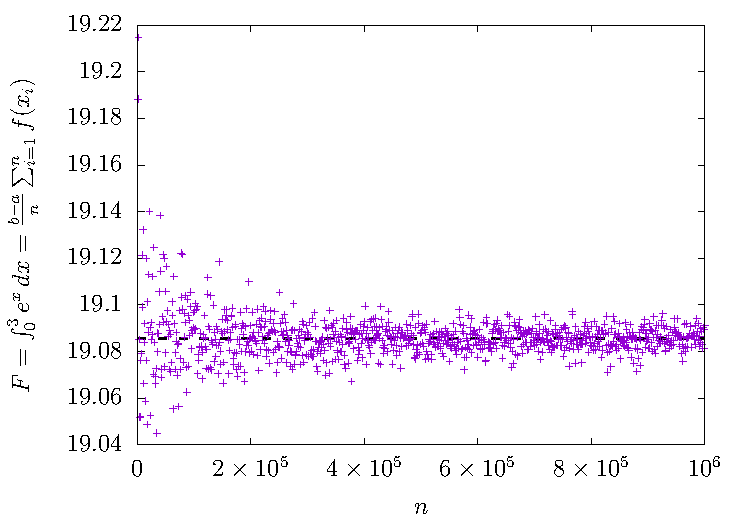
\includegraphics[width=.8\textwidth]{1-I-n.pdf}
        \caption{积分结果$F$随抽取的数据点数量$n$的变化情况,其中的黑色虚线是积分的准确值.}
        \label{1-F-n}
    \end{figure}

    由图\ref{1-F-n}可见,随着抽取的数据点数量$n$增加,Monte Carlo积分结果越来越接近于积分的准确值,这符合中心极限定理.
\end{sol}

\begin{prob}[Sample Mean method for higher dimensional integration. (5 points)]
    Please perform the following three dimensional integration with two different methods: one uses the conventional integration on equally discretized points, the other one uses the Monte Carlo method. By using the same number of points in the two methods, compare the accuracy and speed of the two algorithms.
    \begin{align}
        \int_0^{2\pi}d\phi\int_0^{3a}\rho^3\,d\rho\int_{-\sqrt{9a^2-\rho^2}}^{\sqrt{9a^2-\rho^2}}dz=\frac{648\pi}{5}a^3.
    \end{align}
\end{prob}
\begin{sol}
    取$a=1$.
    \begin{itemize}
        \item \textbf{传统数值积分方法}:用拓展到三维的中矩形公式计算积分,算法如下,代码见附录.
        \begin{enumerate}
            \item 在$\phi\in[0,2\pi],\rho\in[0,3a],z\in[-3a,3a]$范围内均匀取离散点,其中$\phi$和$z$维度离散$N$份,$\rho$维度离散$N\times N_{\text{tasks}}$分($N_{\text{tasks}}$为参与运算的节点数量):
            \begin{align}
                \phi_i=&\left(i-\frac{1}{2}\right)\Delta\phi,\quad\Delta\phi=\frac{2\pi-0}{500}\quad i=1,2,\cdots,500,\\
                \rho_j=&\left(j-\frac{1}{2}\right)\Delta\rho,\quad\Delta\rho=\frac{3a-0}{500},\quad j=1,2,\cdots,500,\\
                z_k=&-3a+\left(k-\frac{1}{2}\right)\Delta z,\quad\Delta z=\frac{3a-(-3a)}{500},\quad k=1,2,\cdots,500.
            \end{align}
            \item 计算各个离散点上的函数值:
            \begin{align}
                f(\phi_i,\rho_j,z_k)=\rho_j^3,
            \end{align}
            其中第$n$个节点计算标号为$i=1,2,\cdots,N,\quad j=0\times N_{\text{tasks}}+n,1\times N_{\text{tasks}}+n,\cdots,(N-1)N_{\text{tasks}}+n,\quad k=1,2,\cdots,N$的离散点(共$N^3$个)上的函数值.
            \item 判断各个离散点是否处于$\phi\in[0,2\pi],\rho\in[0,3a],z\in[-\sqrt{9a^2-\rho^2},\sqrt{9a^2-\rho^2}]$这一积分范围内,用指标$H$来表示:
            \begin{align}
                H(\phi_i,\rho_j,z_k)=\left\{\begin{array}{ll}
                    1,&\phi_i\in[0,2\pi],\rho_j\in[0,3a],z_k\in[-\sqrt{9a^2-z^2},\sqrt{9a^2-z^2}],\\
                    0,&\text{otherwise}.
                \end{array}\right.
            \end{align}
            \item 将所有处于积分范围内的离散点上的函数值求和取平均并乘上积分范围的体积,得到数值积分结果:
            \begin{align}
                I\approx\left(\frac{2\pi-0}{N}\right)\left(\frac{3a-0}{N}\right)\left(\frac{3a-(-3a)}{N}\right)\sum_{i=1}^{N}\sum_{j=1}^{N}\sum_{k=1}^{N}f(\phi_i,\rho_j,z_k)H(\phi_i,\rho_j,z_k).
            \end{align}
            \item 用CPU\_TIME来得到各个节点的计算耗时,将所有节点的计算耗时加和得到计算总耗时,将计算结果与积分的准确值$\frac{648\pi}{5}a^3$做差得到计算误差.
        \end{enumerate}
        \item \textbf{Monte Carlo方法}:
        \begin{itemize}
            \item \textbf{Sample mean方法}:算法与前一题题干中针对一维情况的大体相同,代码见附录
            \begin{enumerate}
                \item $N_{\text{tasks}}$个具有不同seed的节点参与运算,每个节点在$\phi\in[0,2\pi],\rho\in[0,3\pi],z\in[-3a,3a]$范围内均匀随机抽取$N^3$个点.
                \item 计算各个随机抽取的点上的函数值:
                \begin{align}
                    f(\phi_{n,i},\rho_{n,i},z_{n,i})=\rho_{n,i}^3.
                \end{align}
                其中$n=0,1,\cdots,N_{\text{tasks}}-1$代表CPU节点的序号,$i=1,2,\cdots,N$代表随机抽取的点的序号.
                \item 判断各个离散点是否处于$\phi\in[0,2\pi],\rho\in[0,3a],z\in[-\sqrt{9a^2-\rho^2},\sqrt{9a^2-\rho^2}]$这一积分范围内,用指标$H$来表示:
                \begin{align}
                    H(\phi_{n,i},\rho_{n,i},z_{n,i})=\left\{\begin{array}{ll}
                        1,&\phi_{n,i}\in[0,2\pi],\rho_{n,i}\in[0,3a],z_{n,i}\in[-\sqrt{9a^2-z^2},\sqrt{9a^2-z^2}],\\
                        0,&\text{otherwise}.
                    \end{array}\right.
                \end{align}
                \item 将所有处于积分范围内的离散点上的函数值求和取平均并乘上积分范围的体积,得到数值积分结果:
                \begin{align}
                    I\approx\frac{1}{N_{\text{tasks}}}\left(\frac{2\pi-0}{N}\right)\left(\frac{3a-0}{N}\right)\left(\frac{3a-(-3a)}{N}\right)\sum_{n=0}^{N_{\text{tasks}}-1}\sum_{i=1}^{N^3}f(\phi_{n,i},\rho_{n,i},z_{n,i})H(\phi_{n,i},\rho_{n,i},z_{n,i}).
                \end{align}
                \item 用CPU\_TIME来得到各个节点的计算耗时,将所有节点的计算耗时加和来作为计算总耗时,以积分的准确值$\frac{648\pi}{5}a^3$为平均值计算所有节点计算结果的标准差来作为计算误差:
                \small
                \begin{align}
                    \sigma=\left[\frac{1}{N_{\text{tasks}}}\sum_{n=0}^{N_{\text{tasks}}-1}\left(I_n-\frac{648\pi}{5}a^3\right)^2\right]^{1/2}.
                \end{align}
                其中
                \begin{align}
                    I_n=\left(\frac{2\pi}{N}\right)\left(\frac{3a-0}{N}\right)\left(\frac{3a-(-3a)}{N}\right)\sum_{i=1}^{N^3}f(\phi_{n,i},\rho_{n,i},z_{n,i})H(\phi_{n,i},\rho_{n,i},z_{n,i})
                \end{align}
                是标号为$n$的节点计算得到的积分值.
                \normalsize
            \end{enumerate}
            \item \textbf{Hit-or-Miss方法}:算法如下,代码见附录.
            \begin{enumerate}
                \item $N_{\text{tasks}}$个具有不同seed的节点参与运算,每个节点在$\phi\in[0,2\pi],\rho\in[0,3\pi],z\in[-3a,3a],f\in[0,27a^3]$范围内均匀随机抽取$N^3$个点.
                \item 每个节点计算各自的$N^3$个点中满足
                \begin{align}
                    f_{n,i}<\rho_{n,i}^3,
                \end{align}
                并且在积分范围内
                \begin{align}
                    \phi_{n,i}\in[0,2\pi],\quad\rho_{n,i}\in[0,3a],\quad z_{n,i}\in[-\sqrt{9a^2-\rho^2},\sqrt{9a^2-\rho^2}],
                \end{align}
                的点数$n_{\text{in},n}$.
                \item 用下式计算数值积分结果:
                \begin{align}
                    I\approx\frac{1}{N_{\text{tasks}}}\sum_{n=0}^{N_{\text{tasks}}-1}\frac{n_{\text{in},i}}{N}\left(\frac{2\pi-0}{N}\right)\left(\frac{3a-0}{N}\right)\left(\frac{3a-(-3a)}{N}\right)(27a^3-0).
                \end{align}
                \item 用CPU\_TIME来得到各个节点的计算耗时,将所有节点的计算耗时加和来作为计算总耗时,以积分的准确值$\frac{648\pi}{5}a^3$为平均值计算所有节点计算结果的标准差来作为计算误差:
                \begin{align}
                    \sigma=\left[\frac{1}{N_{\text{tasks}}}\sum_{n=0}^{N_{\text{tasks}}-1}\left(I_n-\frac{648\pi}{5}a^3\right)^2\right]^{1/2}.
                \end{align}
                其中
                \begin{align}
                    I_n=\sum_{i=1}^{N^3}\frac{n_{\text{in},n}}{N}\left(\frac{2\pi-0}{N}\right)\left(\frac{3a-0}{N}\right)\left(\frac{3a-(-3a)}{N}\right)(27a^3-0).
                \end{align}
            \end{enumerate}
        \end{itemize}
    \end{itemize}
    统一选取$a=1,N=500,n_{\text{tasks}}=16$(也就是说三种方法都是总共对$500^3\times 16$个点进行了计算)来测试上述三种方法,其计算结果、总耗时、计算误差如表\ref{2-T}.

    \begin{table}[h]
        \centering
        \caption{测试结果汇总.}
        \label{2-T}
        \begin{tabular}{c|ccc}
        选用的积分方法 & 计算结果 & 总耗时(s) & 计算误差 \\ \hline
        传统数值积分方法 & 407.14869 & 40.91978 & -0.00171 \\
        Sample mean方法 & 407.15133 & 342.42996 & 0.00532 \\
        Hit-or-Miss方法 & 407.12599 & 433.94705 & 0.01177
        \end{tabular}
    \end{table}

    可见在积分只有三维的情况下,传统数值积分方法的速度和精度都尚优于Monte Carlo方法. 其实仔细研究传统数值积分方法和sample mean算法的代码,可以发现两者的主要区别就在于选取离散点的方法,前者通过循环均匀遍历积分的区间,而后者通过随机数发生器随机抽取积分范围内的点,所以推测导致后者比前者耗时更多的原因是调用随机数发生器会消耗较多的资源. Hit-or-Miss方法比sample mean方法更耗时间,是因为后者只需要计算随机抽取的点上的函数值即可,而前者不仅要计算随机抽取的点上的函数值,而且还要将猜测的函数值与真实的函数值进行比较. Hit-or-Miss方法也比sample mean方法精度更差,这是因为对于每个随机抽取的点,后者精确地计算了该点的函数值,而前者仅得到了猜测的函数值与真实的函数的大小关系这一信息,显然是前者在模拟中获得的信息更多,因而精度更高.

    当然,对于更高维度的积分,传统数值积分方法的资源消耗可能会大幅增加,这时可能Monte Carlo积分方法更为适用.
\end{sol}

\section*{附录}
\textbf{Problem 1 sample mean算法Fortran代码}
\begin{lstlisting}
program main
    use mpi
    implicit none
    integer :: ntasks, rank, ierr
    integer, allocatable :: status(:)
    integer :: clock, n
    integer, allocatable :: seed(:)
    integer(4) :: i, n_tot
    real(8), parameter :: l = 0.d0, r = 3.d0
    real(8) :: x, y
    real(8) :: integral_local, integral

    ! initialize the MPI environment
    call MPI_INIT(ierr)
    call MPI_COMM_SIZE(MPI_COMM_WORLD, ntasks, ierr)
    call MPI_COMM_RANK(MPI_COMM_WORLD, rank, ierr)
    allocate(status(MPI_STATUS_SIZE))

    ! initialize the random number for different processes
    if (rank == 0) then
        call SYSTEM_CLOCK(clock)
        call RANDOM_SEED(size = n)
        allocate(seed(n))
        do i = 1, n
            seed(i) = clock + 37 * i
        end do
        call RANDOM_SEED(PUT = seed)
        deallocate(seed)
        do i = 1, ntasks - 1
            call RANDOM_NUMBER(x)
            clock = clock + Int(x * 1000000)
            call MPI_SEND(clock, 1, MPI_INTEGER, i, i, MPI_COMM_WORLD, ierr)
        end do
        open(unit = 1, file = '1-I-n.txt', status = 'unknown')
    else
        call MPI_RECV(clock, 1, MPI_INTEGER, 0, rank, MPI_COMM_WORLD, status, ierr)
        call RANDOM_SEED(size = n)
        allocate(seed(n))
        do i = 1, n
            seed(i) = clock + 37 * i
        end do
        call RANDOM_SEED(PUT = seed)
        deallocate(seed)
    end if

    do n_tot = 1000, 1000000, 1000
        integral_local = 0.d0
        integral = 0.d0
        do i = 1, n_tot
            call RANDOM_NUMBER(x)
            x = x * (r - l) + l
            call func(x, y)
            integral_local = integral_local + y
        end do
        integral_local = (r - l) * integral_local / dble(n_tot)

        call MPI_REDUCE(integral_local, integral, 1, MPI_REAL8, MPI_SUM, 0, MPI_COMM_WORLD, ierr)

        if (rank == 0) then
            integral = integral / dble(ntasks)
            write(1,'(i10,f10.5)') n_tot, integral
        end if
    end do

    if (rank == 0) then
        close(1)
    end if

    call MPI_FINALIZE(ierr)
end program main

subroutine func(x, y)
    ! the function to be integrated
    implicit none
    real(8), intent(in) :: x
    real(8), intent(out) :: y

    y = exp(x)
end subroutine func
\end{lstlisting}

\textbf{Problem 2 传统数值积分方法计算积分Fortran代码}
\begin{lstlisting}
    program main
    use mpi
    implicit none
    integer :: ntasks, rank, ierr
    integer, allocatable :: status(:)
    integer, parameter :: n = 500
    integer :: i, j, k
    real(8), parameter :: pi = acos(-1.d0)
    real(8), parameter :: phi_l = 0.d0, phi_u = 2 * pi, rho_l = 0.d0, rho_u = 3.d0, z_l = -3.d0, z_u = 3.d0
    real(8), parameter :: d_phi = (phi_u - phi_l) / dble(n), d_rho = (rho_u - rho_l) / dble(n), d_z = (z_u - z_l) / dble(n)
    real(8) :: phi, rho, z, f, H
    real(8) :: integral_local = 0.d0, integral
    real :: start, finish, time


    ! initialize the MPI environment
    call MPI_INIT(ierr)
    call MPI_COMM_SIZE(MPI_COMM_WORLD, ntasks, ierr)
    call MPI_COMM_RANK(MPI_COMM_WORLD, rank, ierr)
    allocate(status(MPI_STATUS_SIZE))

    call CPU_TIME(start)

    phi = phi_l - d_phi / dble(2)
    do i = 1, n
        phi = phi + d_phi
        rho = rho_l - d_rho + d_rho / dble(ntasks) / dble(2) + d_rho / dble(ntasks) * dble(rank)
        do j = 1, n
            rho = rho + d_rho
            z = z_l - d_z / dble(2)
            do k = 1, n
                z = z + d_z
                call func(phi, rho, z, f)
                call inArea(phi, rho, z, H)
                integral_local = integral_local + f * H
            end do
        end do
    end do
   
    call MPI_REDUCE(integral_local, integral, 1, MPI_REAL8, MPI_SUM, 0, MPI_COMM_WORLD, ierr)

    if (rank == 0) then
        integral = (phi_u - phi_l) * (rho_u - rho_l) * (z_u - z_l) / dble(ntasks) / dble(n**3) * integral
        write(*,'(f10.5)') integral
    end if

    call CPU_TIME(finish)
    call MPI_REDUCE(finish - start, time, 1, MPI_REAL, MPI_SUM, 0, MPI_COMM_WORLD, ierr)
    if (rank == 0) then
        write(*,'(f10.5)') time
    end if

    call MPI_FINALIZE(ierr)
end program main

subroutine func(phi, rho, z, f)
    ! the function to be integrated
    implicit none
    real(8), intent(in) :: phi, rho, z
    real(8), intent(out) :: f

    f = rho**3
end subroutine func

subroutine inArea(phi, rho, z, H)
    ! judge whether the dot is in the integral area
    real(8), intent(in) :: phi, rho, z
    real(8), intent(out) :: H

    if ((z > -sqrt(9.d0 - rho**2)) .and. (z < sqrt(9.d0 - rho**2))) then
        H = 1.d0
    else
        H = 0.d0
    end if
end subroutine inArea
\end{lstlisting}
\textbf{Problem 2 sample mean算法Fortran代码}
\begin{lstlisting}
    program main
    use mpi
    implicit none
    integer :: ntasks, rank, ierr
    integer, allocatable :: status(:)
    integer :: clock, n
    integer, allocatable :: seed(:)
    integer(4) :: i, n_tot = 125000000
    real(8), parameter :: pi = acos(-1.d0)
    real(8), parameter :: phi_l = 0.d0, phi_u = 2.d0 * pi, rho_l = 0.d0, rho_u = 3.d0, z_l = -3.d0, z_u = 3.d0
    real(8) :: phi, rho, z, f, H
    real(8) :: integral_local = 0.d0, integral
    real :: start, finish, time
    real(8) :: sigma

    ! initialize the MPI environment
    call MPI_INIT(ierr)
    call MPI_COMM_SIZE(MPI_COMM_WORLD, ntasks, ierr)
    call MPI_COMM_RANK(MPI_COMM_WORLD, rank, ierr)
    allocate(status(MPI_STATUS_SIZE))

    call CPU_TIME(start)

    ! initialize the random number for different processes
    if (rank == 0) then
        call SYSTEM_CLOCK(clock)
        call RANDOM_SEED(size = n)
        allocate(seed(n))
        do i = 1, n
            seed(i) = clock + 37 * i
        end do
        call RANDOM_SEED(PUT = seed)
        deallocate(seed)
        do i = 1, ntasks - 1
            call RANDOM_NUMBER(z)
            clock = clock + Int(z * 1000000)
            call MPI_SEND(clock, 1, MPI_INTEGER, i, i, MPI_COMM_WORLD, ierr)
        end do
    else
        call MPI_RECV(clock, 1, MPI_INTEGER, 0, rank, MPI_COMM_WORLD, status, ierr)
        call RANDOM_SEED(size = n)
        allocate(seed(n))
        do i = 1, n
            seed(i) = clock + 37 * i
        end do
        call RANDOM_SEED(PUT = seed)
        deallocate(seed)
    end if

    do i = 1, n_tot
        call RANDOM_NUMBER(phi)
        phi = phi * (phi_u - phi_l) + phi_l
        call RANDOM_NUMBER(rho)
        rho = rho * (rho_u - rho_l) + rho_l
        call RANDOM_NUMBER(z)
        z = z * (z_u - z_l) + z_l
        call func(phi, rho, z, f)
        call inArea(phi, rho, z, H)
        integral_local = integral_local + f * H
    end do
    integral_local = (phi_u - phi_l) * (rho_u - rho_l) * (z_u - z_l) / dble(n_tot) * integral_local

    call MPI_REDUCE(integral_local, integral, 1, MPI_REAL8, MPI_SUM, 0, MPI_COMM_WORLD, ierr)

    if (rank == 0) then
        integral = integral / dble(ntasks)
        write(*,'(f10.5)') integral
    end if

    call CPU_TIME(finish)
    call MPI_REDUCE(finish - start, time, 1, MPI_REAL, MPI_SUM, 0, MPI_COMM_WORLD, ierr)
    if (rank == 0) then
        write(*,'("Time consumed: ",f10.5)') time
    end if
    call MPI_REDUCE(((integral_local - dble(648) * pi / dble(5))**2)**2, sigma, 1, MPI_REAL8, MPI_SUM, 0, MPI_COMM_WORLD, ierr)
    if (rank == 0) then
        write(*,'("Error: ",f10.5)') sqrt(sigma / dble(ntasks))
    end if

    call MPI_FINALIZE(ierr)
end program main

subroutine func(phi, rho, z, f)
    ! the function to be integrated
    implicit none
    real(8), intent(in) :: phi, rho, z
    real(8), intent(out) :: f

    f = rho**3
end subroutine func

subroutine inArea(phi, rho, z, H)
    ! judge whether the dot is in the integral area
    real(8), intent(in) :: phi, rho, z
    real(8), intent(out) :: H

    if ((z > -sqrt(9.d0 - rho**2)) .and. (z < sqrt(9.d0 - rho**2))) then
        H = 1.d0
    else
        H = 0.d0
    end if
end subroutine inArea
\end{lstlisting}
\textbf{Problem 2 hit-or-miss算法Fortran代码}
\begin{lstlisting}
    program main
    use mpi
    implicit none
    integer :: ntasks, rank, ierr
    integer, allocatable :: status(:)
    integer :: i, n, clock
    integer, allocatable :: seed(:)
    real(8), parameter :: pi = acos(-1.d0)
    integer(4) :: n_in_local = 0, n_in, n_tot = 125000000
    real(8), parameter :: phi_l = 0.d0, phi_u = 2 * pi, rho_l = 0.d0, rho_u = 3.d0, z_l = -3.d0, z_u = 3.d0,&
        f_l = 0.d0, f_u = 27.d0
    integer :: H
    real(8) :: phi, rho, z, f, f_real
    real(8) :: integral_local, integral
    real :: start, finish, time
    real(8) :: sigma

    ! initialize the MPI environment
    call MPI_INIT(ierr)
    call MPI_COMM_SIZE(MPI_COMM_WORLD, ntasks, ierr)
    call MPI_COMM_RANK(MPI_COMM_WORLD, rank, ierr)
    allocate(status(MPI_STATUS_SIZE))

    call CPU_TIME(start)

    if (rank == 0) then
        call SYSTEM_CLOCK(clock)
        call RANDOM_SEED(size = n)
        allocate(seed(n))
        do i = 1, n
            seed(i) = clock + 37 * i
        end do
        call RANDOM_SEED(PUT = seed)
        deallocate(seed)
        do i = 1, ntasks - 1
            call RANDOM_NUMBER(z)
            clock = clock + Int(z * 1000000)
            call MPI_SEND(clock, 1, MPI_INTEGER, i, i, MPI_COMM_WORLD, ierr)
        end do
    else
        call MPI_RECV(clock, 1, MPI_INTEGER, 0, rank, MPI_COMM_WORLD, status, ierr)
        call RANDOM_SEED(size = n)
        allocate(seed(n))
        do i = 1, n
            seed(i) = clock + 37 * i
        end do
        call RANDOM_SEED(PUT = seed)
        deallocate(seed)
    end if

    do i = 1, n_tot
        call RANDOM_NUMBER(phi)
        phi = phi * (phi_u - phi_l) + phi_l
        call RANDOM_NUMBER(rho)
        rho = rho * (rho_u - rho_l) + rho_l
        call RANDOM_NUMBER(z)
        z = z * (z_u - z_l) + z_l
        call RANDOM_NUMBER(f)
        f = f * (f_u - f_l) + f_l
        call func(phi, rho, z, f_real)
        call inArea(phi, rho, z, H)
        if (f < f_real) then
            n_in = n_in + H
        end if
    end do
    integral_local = (phi_u - phi_l) * (rho_u - rho_l) * (z_u - z_l) * (f_u - f_l) * dble(n_in) / dble(n_tot)

    call MPI_REDUCE(integral_local, integral, 1, MPI_REAL8, MPI_SUM, 0, MPI_COMM_WORLD, ierr)

    if (rank == 0) then
        integral = integral / dble(ntasks)
        write(*,'(f10.5)') integral
    end if

    call CPU_TIME(finish)
    call MPI_REDUCE(finish - start, time, 1, MPI_REAL, MPI_SUM, 0, MPI_COMM_WORLD, ierr)
    if (rank == 0) then
        write(*,'("Time consumed: "f10.5)') time
    end if
    call MPI_REDUCE(((integral_local - dble(648) * pi / dble(5))**2)**2, sigma, 1, MPI_REAL8, MPI_SUM, 0, MPI_COMM_WORLD, ierr)
    if (rank == 0) then
        write(*,'("Error: ",f10.5)') sqrt(sigma / dble(ntasks))
    end if

    call MPI_FINALIZE(ierr)
end program main

subroutine func(phi, rho, z, f)
    ! the function to be integrated
    implicit none
    real(8), intent(in) :: phi, rho, z
    real(8), intent(out) :: f

    f = rho**3
end subroutine func

subroutine inArea(phi, rho, z, H)
    ! judge whether the dot is in the integral area
    real(8), intent(in) :: phi, rho, z
    integer, intent(out) :: H

    if ((z > -sqrt(9.d0 - rho**2)) .and. (z < sqrt(9.d0 - rho**2))) then
        H = 1
    else
        H = 0
    end if
end subroutine inArea
\end{lstlisting}
\end{document}